\section{快速解码的算法方法}
\label{sec:fast-decoding}

\begin{figure*}[h]
    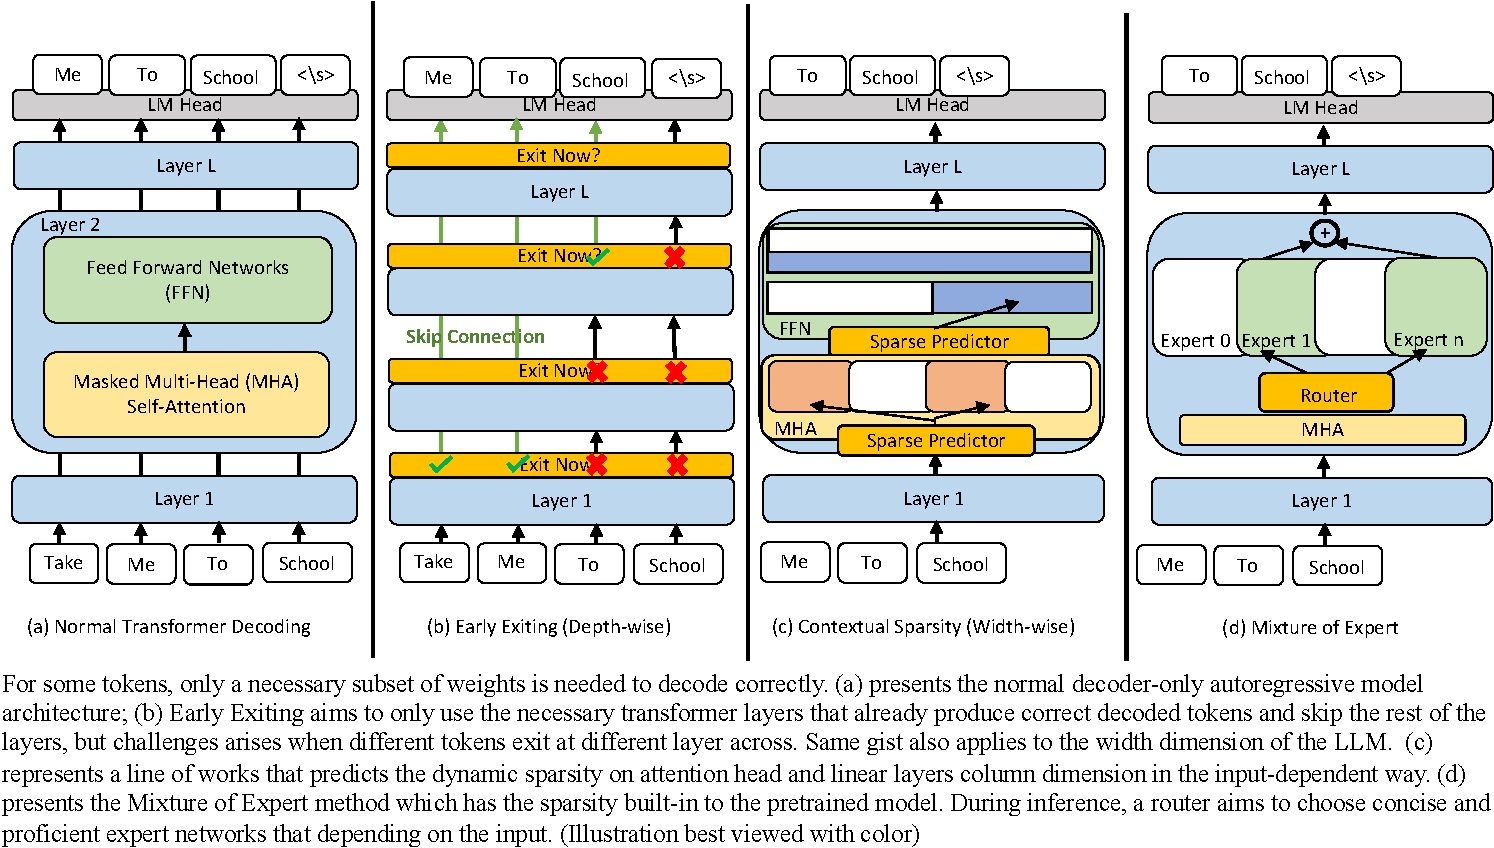
\includegraphics[width=\textwidth]{EarlyExiting.pdf}
    \caption{输入相关动态网络技术示意图}
    \label{fig:early_exiting}
\end{figure*}

LLM 在文本生成任务上表现卓越，但其解码阶段通常按自回归方式逐 token 生成。
每生成一个 token，都需要重复读取解码器权重。
随着模型参数规模增大，解码过程高度 memory-bound~\citep{dejong2023fido}，硬件利用率低，导致时延显著增大~\citep{kim2023stack}。
在 ChatBot 等实时交互场景中，这一问题尤为突出，因此需要专门优化解码过程。

本节从算法角度回顾降低推理成本的方法，主要分两条路径：
\begin{itemize}
    \item 在固定“每个 token 解码”前提下，如何最小化每次解码所需参数量（Sec.~\ref{fixedtoken}）。
    \item 在固定“每次前向使用参数量”前提下，如何最大化单次前向可解码 token 数（Sec.~\ref{fixedparameter}）。
\end{itemize}

\subsection{每个 token 解码所需最小参数}
\label{fixedtoken}

已有研究指出，即使语言模型参数巨大，生成正确 token 并不总需要全部参数~\cite{simoulin-crabbe-2021-many}。
因此可对输入相关地选择参数子集，从而在保持精度的同时降低时延。
本节从三类动态稀疏策略讨论：
(1) 早退（depth/layer 维度动态）；
(2) 上下文稀疏（width 维度动态）；
(3) MoE（训练时即构建稀疏专家结构）。

\subsubsection{早退（Early Exiting）}
\label{earlyexit}

早退思想在编码器模型中已有大量研究~\citep{baierreinio2020node, hou2020dynabert, li2021cascadebert, liu2020fastbert, liu-etal-2022-towards-efficient, schwartz-etal-2020-right, stickland2019bert, xin2020deebert, zhou2020bert, zhu-2021-leebert, schuster2021consistent}。
但解码器场景更复杂：需要在序列级保持一致性，因为后续 token 依赖先前生成结果。

解码器层结构同构，因此每层隐藏状态都可接 LM Head 产生下一 token 分布。
\cite{geva2022transformer} 与 \cite{simoulin-crabbe-2021-many} 观察到：部分 token 在中间层已出现表示饱和，提前退出即可得到与全层一致的 top-1。
这构成了解码器早退可行性的基础。

\cite{elbayad2020depthadaptive} 在机器翻译任务中提出了早期解码器早退框架。
其通用范式是：每层后由置信度模块（固定指标或小 MLP）评估“当前层是否可饱和退出”，满足条件则提前退出并经 LM Head 输出。

围绕该范式，研究主要集中在四个设计点：

\textbf{(1) 如何建模“可退出置信度”}
CALM~\citep{schuster2022confident} 对比了 softmax 置信度、层间隐藏态相似度、层内线性分类器三种方案；实验显示线性分类器在“开销-精度”权衡上最佳。
\citep{bae2023fast} 发现浅层频繁退出会导致输出长度异常，且逐层打分开销高，因此将退出点简化为“浅模块”或“全模型”两选一，减少分类器数量并取得更高加速。
ConsistentEE~\citet{zeng2023consistentee} 则引入 RL 策略网络，联合优化效率与准确率。

\textbf{(2) 退出判据如何设定}
CALM 通过分布无关校准（FWER）给出阈值，且阈值随序列位置指数下降；
\cite{bae2023fast} 将置信度分布建模为 Beta 分布并在线更新；
\cite{zeng2023consistentee} 直接让策略网络输出退出动作。

\textbf{(3) 隐藏状态传播问题}
当某些 token 提前退出、而后续 token 继续深入层时，后层注意力可能缺失先前 token 的 KV。
\cite{elbayad2020depthadaptive} 与 \cite{schuster2022confident} 提出“状态传播”：将早退层隐藏态拷贝到后续缺失层以近似深层状态。
后续工作~\cite{bae2023fast,ding2023efficiency} 发现该近似会损伤性能，并提出在线重算以替代拷贝。
\cite{chen2023eellm} 通过并行全模型流补齐缺失 KV；\cite{din2023jump} 研究用线性桥接层跨层跳跃，平衡精度与开销。
SkipDecode~\cite{delcorro2023skipdecode} 则采取更激进策略：强制更后位置使用更浅层，避免传播并提升速度。

\textbf{(4) 输出分类器训练}
中间层退出需要分类器（共享或分层独立）配合。
\cite{elbayad2020depthadaptive} 使用各层 CE 均值训练；\cite{schuster2022confident} 对深层赋予更高权重；\cite{bae2023fast} 引入动态蒸馏；\cite{rotem2023finding} 与 \cite{ji-etal-2023-early} 指出多目标联合训练会出现梯度冲突并给出缓解策略。
此外，\cite{chen2023eellm} 还从 3D 并行角度优化了早退部署。

\begin{figure*}[ht]
    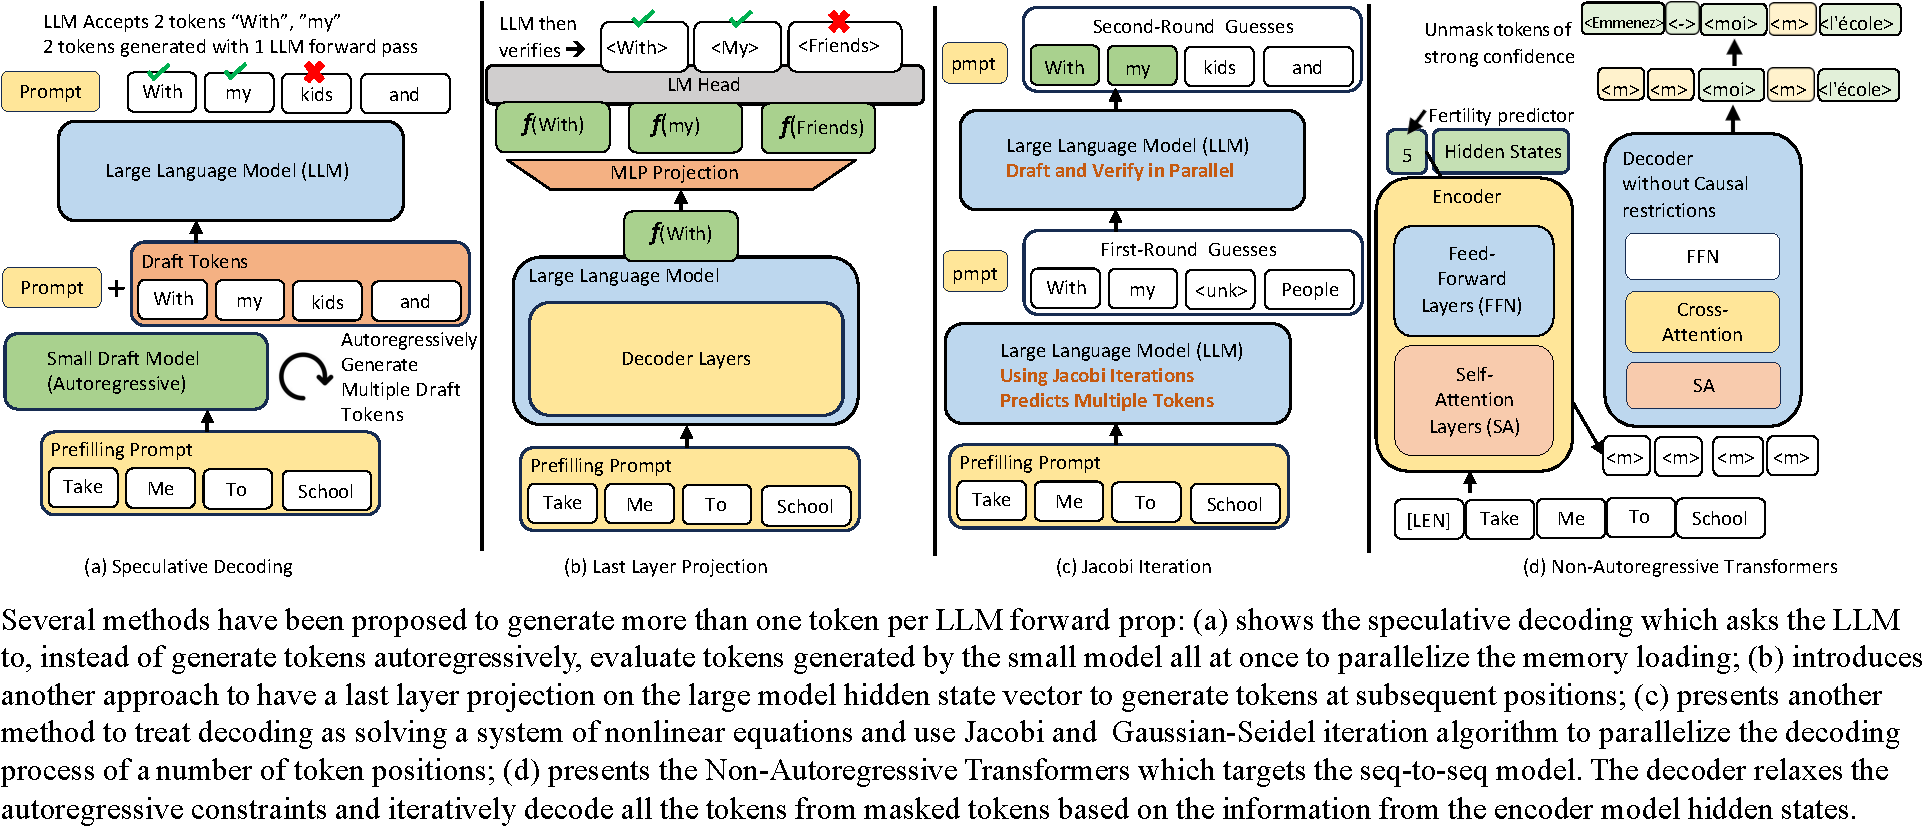
\includegraphics[width=\textwidth]{specudec.pdf}
    \caption{并行解码方法示意图}
    \label{fig:specudec}
\end{figure*}

\subsubsection{上下文稀疏（Contextual Sparsity）}
\label{contextualsparsity}

若早退对应深度维动态稀疏，上下文稀疏则对应宽度维动态稀疏。
Deja Vu~\cite{liu2023deja} 系统研究了 LLM 宽度维动态稀疏，报告上下文稀疏率可达 80\%，即多数权重可在特定 token 下跳过而保持性能。
其核心是为输入 token 动态预测应激活的 attention heads 与 MLP 列，并在 MHA/FFN 前加入小型 Sparse Predictor（图~\ref{fig:early_exiting}(c)），实现超过 2x 推理加速。

PowerInfer~\cite{song2023powerinfer} 将该思路扩展到 CPU+GPU 异构部署，利用“高频激活神经元常驻 GPU、其余驻留 CPU”的策略配合稀疏预测，提升跨设备推理效率。
MatFormer~\cite{devvrit2023matformer} 面向不同硬件能力部署，主要在 FFN 维度做动态结构采样，并通过 Mix’n’Match 形成更灵活模型尺寸。

\subsubsection{专家混合模型（MoE）}
\label{mioe}

语言模型在规模上呈现 power-law 增益~\cite{kaplan2020scaling,hoffmann2022training}，但参数膨胀导致训练与推理效率下降。
MoE~\cite{6215056} 通过“总参数与每次激活计算解耦”提升效率，并可在不显著增加推理计算的前提下扩展模型能力~\cite{lepikhin2020gshard,fedus2021switch}。
如图~\ref{fig:early_exiting}(d)，MoE 用专家网络替换 FFN，并由 gating 为每个 token 选择专家。
更系统内容可见稀疏专家综述~\cite{fedus2022review}。

尽管 MoE 与上下文稀疏都依赖输入决定稀疏结构，但二者不同：
上下文稀疏是在“已训练稠密模型”上挖掘动态稀疏；MoE 则是从训练阶段即构建稀疏模型。

近期 MoE 成果显著：Sparse Mixer~\cite{lee2022sparse}、GLaM~\cite{du2022glam}、ST-MoE~\cite{zoph2022st}、Mixtral 8x7B~\cite{jiang2024mixtral} 等在效率与性能间展现强竞争力。
部署侧也有优化进展，如 RECOMPILE~\cite{kossmann2022optimizing}、MoE 版 ZeRO 推理~\cite{rajbhandari2022deepspeed}、AutoMoE~\cite{jawahar2023automoe}、EdgeMoE~\cite{yi2023edgemoe} 等。

\subsubsection{动态参数缩减的 Roofline 分析}

“每 token 最小参数”类方法通常会同时降低计算与访存。
从 Roofline 角度看，这类方法往往不会显著改变单算子的算术强度与 bound 类型，但会减少总工作量。

对 Early Exiting / Layer Skipping 而言，整层被跳过，故计算、访存、时延通常近似按比例下降；
对 Contextual Sparsity / MoE 而言，不同子算子算术强度差异较大，动态激活模式不同，最终时延收益也会不同。

\subsection{单次前向最大化解码 token 数}
\label{fixedparameter}

另一条降时延路径是放松严格自回归约束，让一次大模型前向尽可能产出多个 token。
本节包括两类：
(1) speculative decoding（用小草稿模型提议候选，大模型验证）；
(2) 直接并行解码（不依赖额外小 Transformer 草稿模型）。

\subsubsection{Speculative Decoding}
\label{specdec}

LLM 解码受权重加载与自回归依赖限制，效率较低。
但较小模型常能在“关键 token 被纠正”的前提下逼近大模型序列~\cite{kim2023speculative}。
因此可让小模型先生成草稿 token，大模型周期性验证/纠正。
尽管大模型会额外验证部分错误草稿，FLOPs 可能增加，但权重加载可在 token 维并行摊薄。
在 memory-bound 主导下，总体时延仍可显著下降。

\textbf{分布一致性：}
\cite{kim2023speculative} 早期提出“草稿-回退-回滚”流程（贪心设置）；
\cite{leviathan2023fast} 与 \cite{chen2023accelerating} 指出在拒绝位置做重采样可在理论上保持与大模型自回归一致分布。

\textbf{构建草稿树：}
草稿序列可接受长度通常有限，越远未来越难猜中。
为提高加速比，一类方法在 batch 方向并行多草稿：
SpecTr~\cite{sun2023spectr}、SpecInfer~\cite{miao2023specinfer}、LLMCAD~\cite{xu2023llmcad} 分别从最优传输重采样、树结构构建与边缘部署流水线角度提升验证效率与接受率。

\textbf{蒸馏与自草稿：}
提升草稿模型与大模型分布一致性是另一关键。
\cite{zhou2023distillspec} 给出“接受率与模型散度”联系并验证蒸馏收益；\cite{liu2023online} 进一步提出在线持续蒸馏以适应域漂移。
\cite{zhang2023draft} 则避免单独草稿模型，通过在大模型内部搜索可跳层子模型作为草稿。

\subsubsection{并行解码（Parallel Decoding）}
\label{pd}

除 speculative decoding 外，另有大量方法直接让大模型一次前向预测多个未来 token：

\textbf{多未来 token 直接预测：}
\cite{stern2018blockwise} 早期在 LM Head 前增加投影层；
Medusa~\cite{cai2024medusa} 将该思路扩展到 decoder-only，并配合树结构并行验证；
PASS~\cite{monea2023pass} 使用 lookahead embeddings；
EAGLE~\cite{li2024eagle} 通过 FeatExtrapolator 预测未来隐藏态并构建验证树。

\textbf{高频 n-gram 检索：}
LLMA~\cite{yang2023inference} 利用“重复短语”现象进行前缀匹配并由 LLM 验证；
REST~\cite{he2023rest} 通过短语库+trie 检索；
\cite{lan2023copy} 则增加检索注意力层按相关性选择候选短语。

\textbf{语言层次结构并行：}
Skeleton-of-Thought~\cite{ning2023skeletonofthought} 先生成提纲再并行扩写要点；
APAR~\cite{liu2024apar} 结合层次软 token 与 Medusa，进一步提升速度。

\textbf{Jacobi / Gauss-Seidel 迭代：}
相关工作表明可用并行迭代近似顺序推理~\cite{pmlr-v139-song21a,ortega2000iterative}。
\cite{santilli2023accelerating} 将其用于机器翻译并行解码；
Lookahead Decoding~\cite{fu2023lookahead} 将其扩展到 LLM，并结合检索复用与定制 attention mask 提升效率。

\textbf{非自回归 Transformer（NAT）：}
NAT 在序列到序列任务上通过并行迭代解码多 token 获得加速，相关研究丰富~\cite{gu2017non,wang2019non,li2019hint,sun2019fast,wei2019imitation,shao2020minimizing,lee2018deterministic,ghazvininejad2019maskpredict,guo-etal-2020-jointly,gu2020fully,savinov2021step}，详见综述~\cite{xiao2023survey}。
其核心是在 decoder 侧放松自回归约束，用掩码序列迭代去噪生成；但该范式依赖编码器条件，向 decoder-only 体系直接迁移仍有难度。
